\chapter{Robotic MIS System Control}

\section{RCM Tracking}
\label{section:rcm-tracking}

This section describes how to use an RCM-error metric in order to implement a control system that makes sure that the laparoscopic tool is always aligned with the fulcrum point and it satisfies the RCM 
constraint. To calculate this error, which can then be used as a feedback signal to a control system, the line of the long axis of the surgical tool must be first defined. To define this line, two points are  calculated using the transformation of the surgical tool, which is attached to the robot's TCP on the end-effector. Let the following be the pose of the surgical tool with respect to the global reference frame
$
{}^UT_{T0} = \begin{bmatrix}
\mathbf{\hat{x}} & \mathbf{\hat{y}} & \mathbf{\hat{z}} & \mathbf{p} \\
0                & 0                & 0                & 1 \\
\end{bmatrix}.
$
Using this pose, let $A,B$ be the points such that 
$
\overrightarrow{O_FA} = \mathbf{p},~ \textrm{and} \quad \overrightarrow{O_FB} = \mathbf{p} + \mathbf{\hat{x}}, 
$
where $O_F$ is the origin point of the fulcrum reference frame. The the line of interest is defined as the line $l$ that passes through the points $A$ and $B$. \\

The alignment error is calculated using a known position and orientation for the second fulcrum reference frame. In real-case scenarios the exact position and orientation of the uncertain fulcrum points are estimated. To model the uncertainty of the pose, the pose message of the fulcrum point includes also a covariance matrix. The ROS message that was used was the \textbf{PoseWithCovarianceStamped} which needs the 
following information (with respect to the global frame) to be fully defined:
$
( \mathbf{p}, \mathbf{q}, \mathbf{C} ), \quad \mathbf{p} \in \mathbb{R}^3, \mathbf{q} \in \mathbb{H}, \mathbf{C} \in \mathbb{R}^{6 \times 6},
$
where 
\begin{equation}
\mathbf{C} = \begin{bmatrix}
σ_{xx} & σ_{xy} & σ_{xz} & σ_{xψ} & σ_{xθ} & σ_{xφ} \\
σ_{xy} & σ_{yy} & σ_{yz} & σ_{yψ} & σ_{yθ} & σ_{yφ} \\
σ_{xz} & σ_{yy} & σ_{zz} & σ_{zψ} & σ_{zθ} & σ_{zφ} \\
σ_{xψ} & σ_{yψ} & σ_{zψ} & σ_{ψψ} & σ_{ψθ} & σ_{ψφ} \\
σ_{xθ} & σ_{yθ} & σ_{zθ} & σ_{ψθ} & σ_{θθ} & σ_{θφ} \\
σ_{xφ} & σ_{yφ} & σ_{zφ} & σ_{ψφ} & σ_{θφ} & σ_{φφ} \\
\end{bmatrix}
\end{equation}
The covariance matrix and its coefficients can be calculated using %equations \ref{eq:cov-matrix} and \ref{eq:cov-matrix-coeff}, using t
he mean values of the estimations of $x,y,z,ψ,θ,φ$.

\begin{center}
\begin{figure}[htbp]
\centering
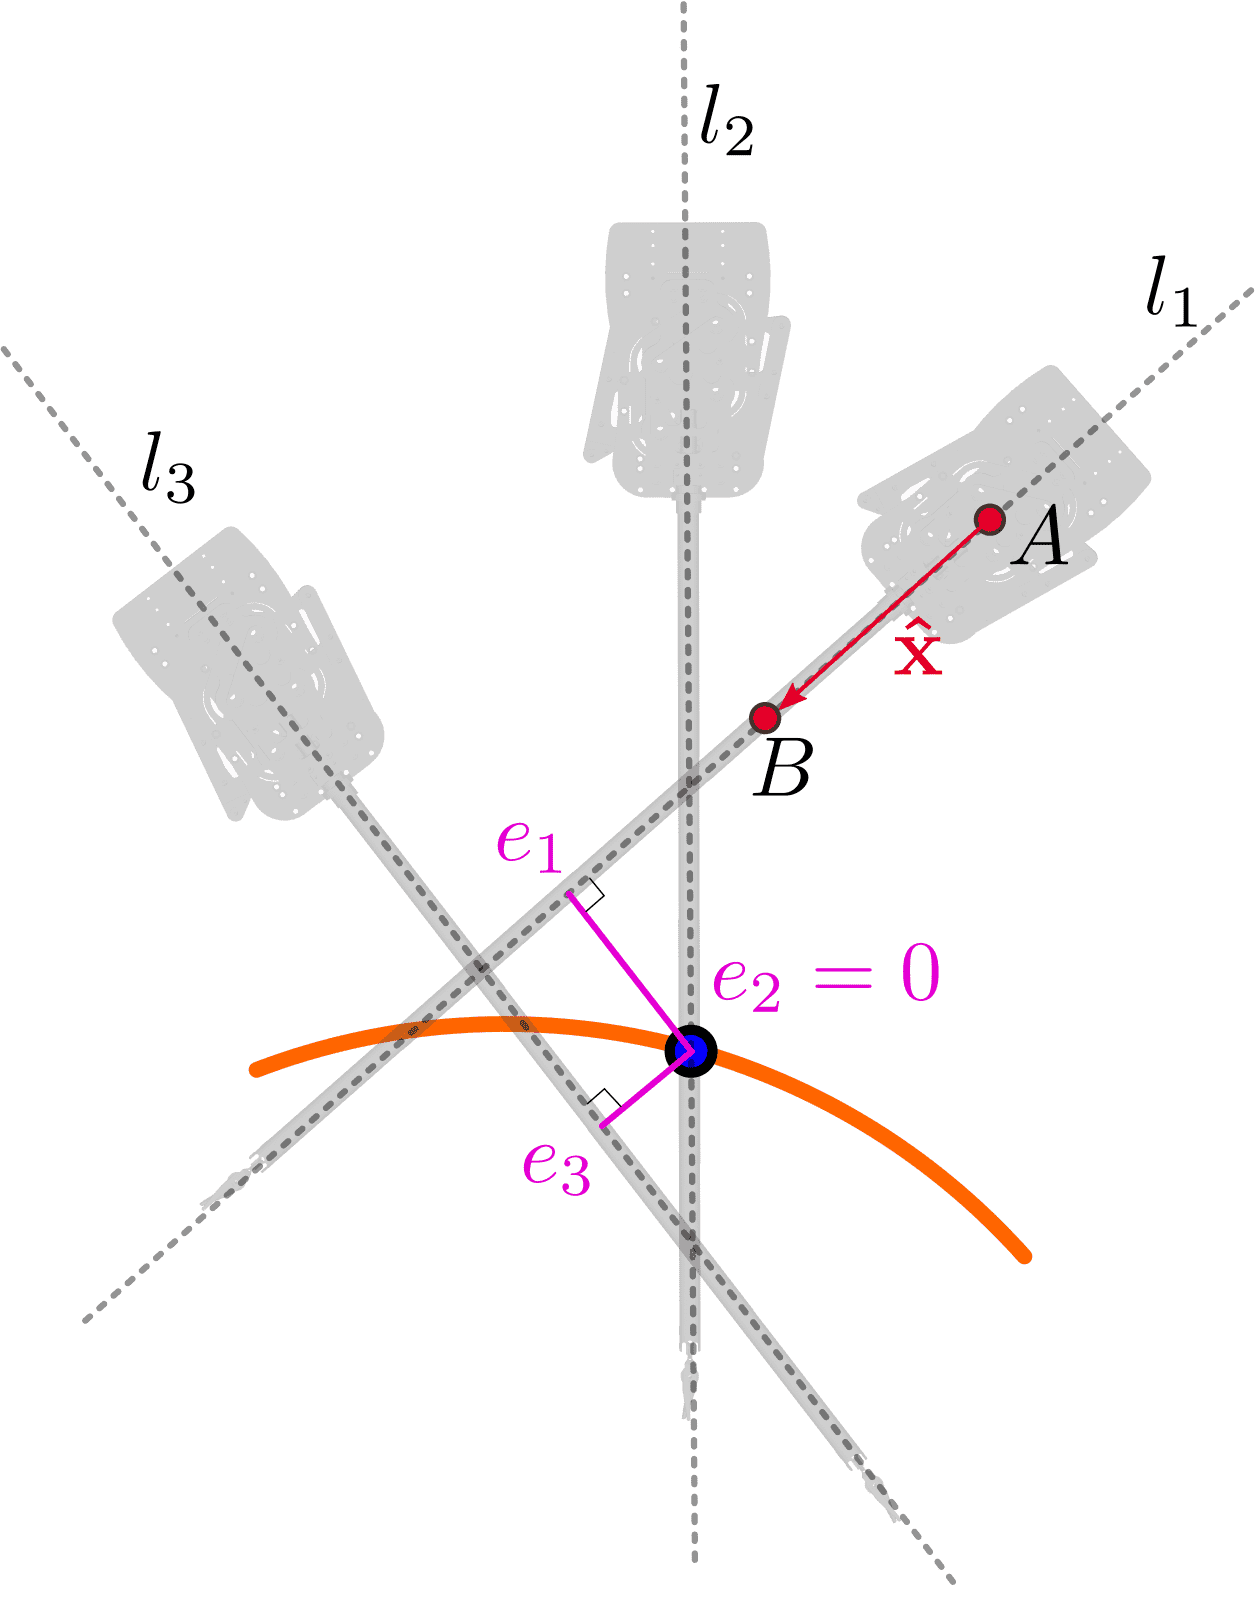
\includegraphics[width=0.5\textwidth]{images/robot_planner6/rcm-error-geometry.png}
\caption{Geometric calculation of the RCM alignment error $e$ using the distance between the line $l$ and the RCM point.}
\label{rcm-error-geometry}
\end{figure}
\end{center}

Since both the origin of the fulcrum reference frame and the line of the long axis of the tool are known then the alignment error can be calculated as the distance of the line $l$ from the point $O_F$
$
e_{rcm} = d(l, O_F).
$

To calculate the distance $d(l, O_F)$ there is available a method in the \textbf{Eigen} C++ library that calculates the distance of a line that passes through 2 points, from a third point. Alternatively, this distance can be calculated using \ref{line-point-distance-formula}.
\begin{equation}
\label{line-point-distance-formula}
d(l, O_F) = \frac{\Vert \overrightarrow{O_FA} \times \mathbf{\hat{x}} \Vert}{\Vert \mathbf{\hat{x}} \Vert}.
\end{equation}
Similar approaches to calculate this error/distance are presented in bibliography \cite{Dong2016RobustTD,Bauzano2009ControlMF}.

If $e_{rcm} \leq 3_{\max} = 1$mm then the surgical tool axis passes through the fulcrum point and executes RCM trajectories, otherwise the robot is considered to have slipped from alignment, it does not execute RCM motion and probably generates a force $f \propto e$ which exerts pressure to the incision point and the abdominal wall (or the tissue around the incision point), which can have negative side-effects in the recovery of the incision. In~\cite{Bauzano2009ControlMF} a different distance $e_s$ is calculated as the RCM error as shown in Figure~\ref{rcm-force-interaction-model}, which is along the x-axis of the fulcrum reference frame or the axis of the abdominal wall. Using this deviation distance $e_s$ the force interaction between the surgical tool and the abdominal wall is $\Vert \mathbf{f}_s \Vert = λ e_s$, where $λ$ is the elasticity of the abdominal wall and can be measured experimentally and $e_s = \frac{1}{cosγ} e.$

\begin{center}
\begin{figure}[htbp]
\centering
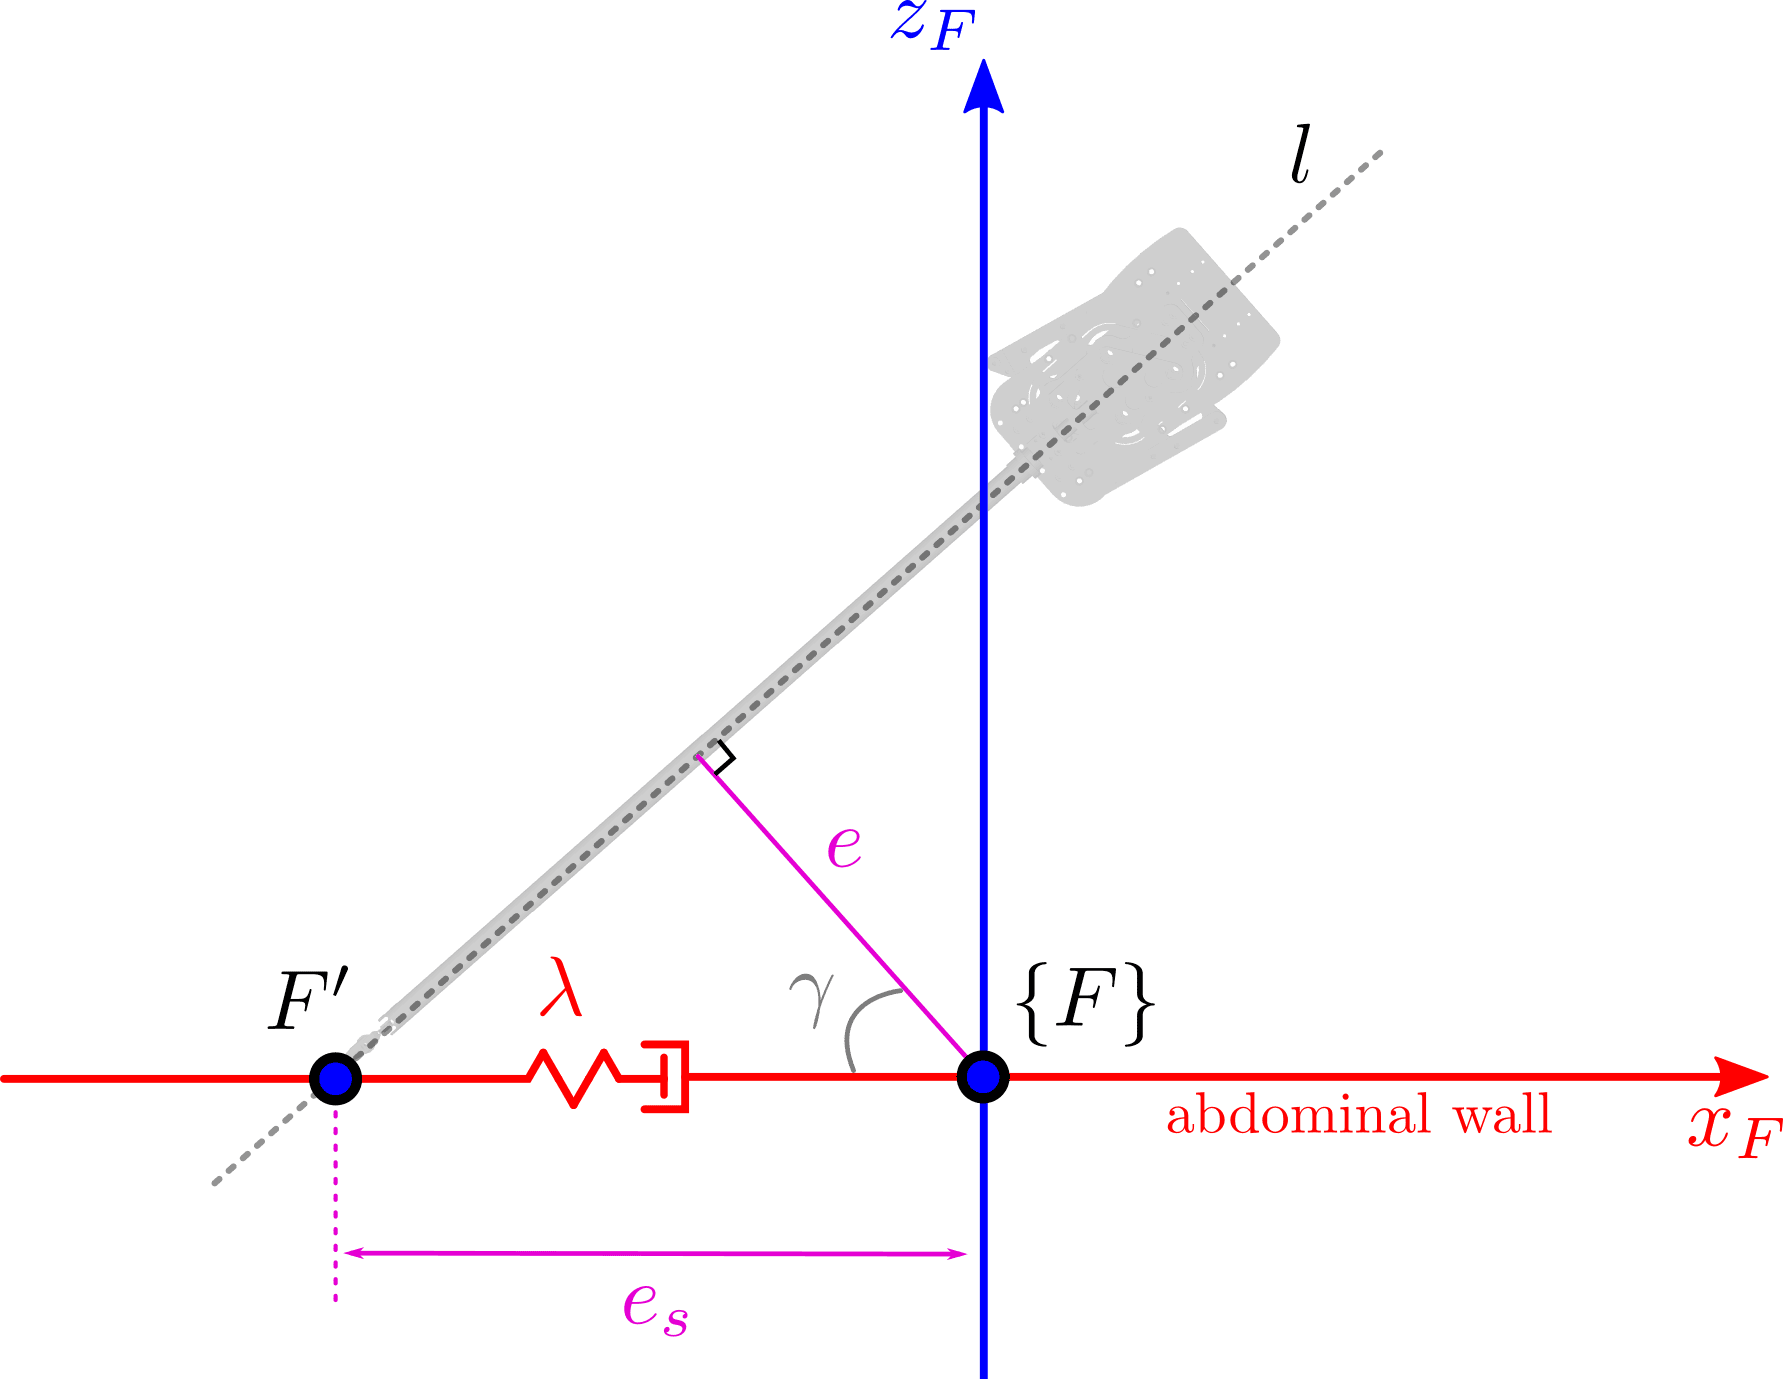
\includegraphics[width=0.4\textwidth]{images/rcm-force-interaction-model.png}
\caption{Force interaction model of the laparoscopic tool and the abdominal wall around the fulcrum point (RCM point)}
\label{rcm-force-interaction-model}
\end{figure}
\end{center}

\begin{center}
\begin{figure}[htbp]
\centering
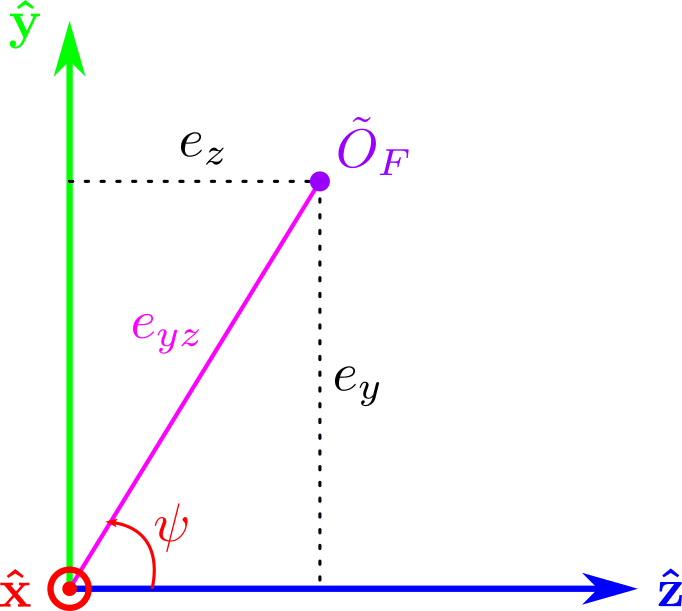
\includegraphics[width=0.4\textwidth]{images/rcm-error-yz.png}
\caption{RCM error calculation in yz plane. The RCM error or yz-error is the distance between the line of the $\mathbf{\hat{x}}$ vector (here seen as a point) and the estimated position of the origin of the fulcrum reference frame $\tilde{O}_F$}
\label{rcm-error-yz-plane}
\end{figure}
\end{center}

The error $e_{rcm}$ can provide further information if the distance of the line $l$ (or of the $\mathbf{\hat{x}}$ axis) from the fulcrum point, is seen from a different perspective than that of 
Figure~\ref{rcm-error-geometry}. If this distance is seen from a plane that is perpendicular to $\mathbf{\hat{x}}$, then the line is seen as a point and the distance $d(l, O_F)$ is seen as a distance between 2 points, as illustrated in Figure~\ref{rcm-error-yz-plane}. This perspective of the RCM error (will also be referenced as yz-error $e_{yz}$) is more useful because it decomposes the error distance in 2 components that can be used to correct the goal pose of the robot so that is fixes the RCM misalignment, as in $e_y = e_{yz}sinψ \quad \textrm{and} \quad e_z = e_{yz}cosψ.~$ The angle $ψ$ that is used to split $e_{rcm}$ in the two components, is already known from the robot's pose and it is the yaw (also known as spin) angle of the surgical tool.

Using the estimated RCM error $\tilde{e}_{rcm}$ and the estimated position of the origin of the fulcrum reference frame, an adaptive motion control system can be designed that corrects the trajectory to avoid RCM misalignment. The proposed control system is illustrated in block diagram~\ref{rcm-control-system-block-diagram} following along a similar pivoting motion control system in \cite{Muoz2005PivotingMC}.

\begin{center}
\begin{figure}[htbp]
\centering
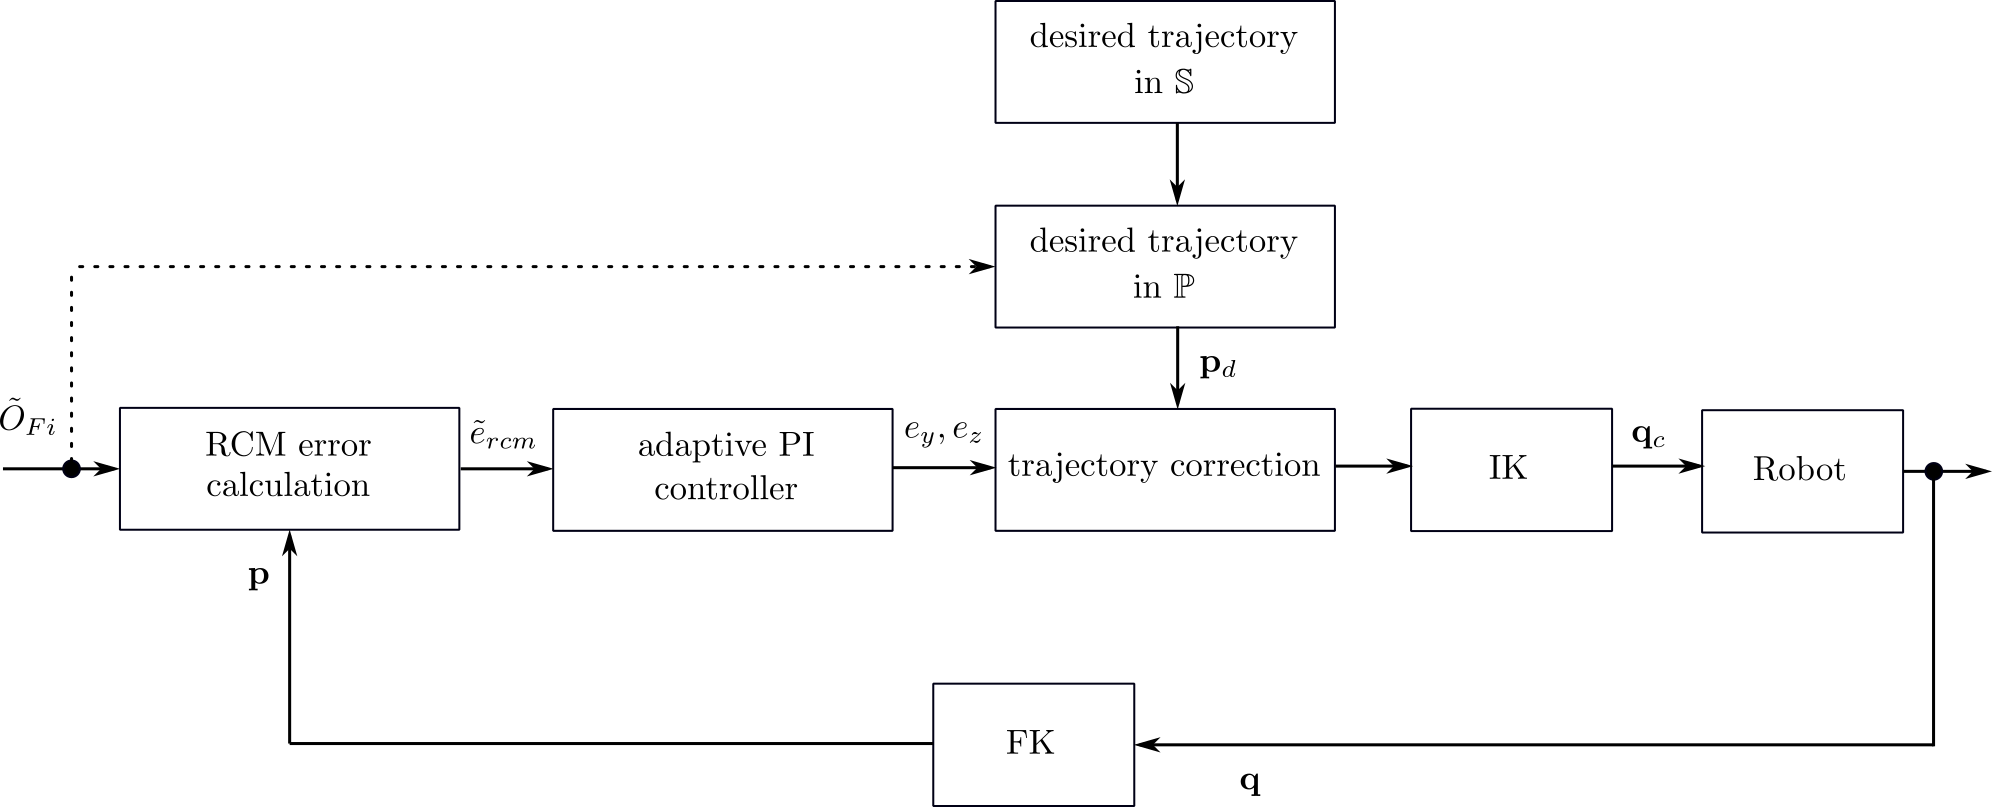
\includegraphics[width=0.8\textwidth]{images/rcm-system-control.png}
\caption{RCM tracking proposed control system.}
\label{rcm-control-system-block-diagram}
\end{figure}
\end{center}

%
\section{Visual Servoing}
%
%At this chapter we briefly investigate how visual servoing can be applied in surgery robotics. \textbf{Visual Servoing} is the use of visual information to guide and control a robot. The main task of visual servoing is to control the end-effector's pose using features extracted from visual information. The features that are usually extracted from cameras are the position and orientation of the detected object, the distance of the object from the camera (using stereoscopic vision, photogrammetry or other techniques), the size and the shape of the object. The visual servoing can be executed either in the robot's space using position-based servoing or in the camera's space (also known as "pixel space") by using the image-based technique.
%
\subsection{Position based servoing}
\clearpage

\begin{center}
\begin{figure}[htbp]
\centering
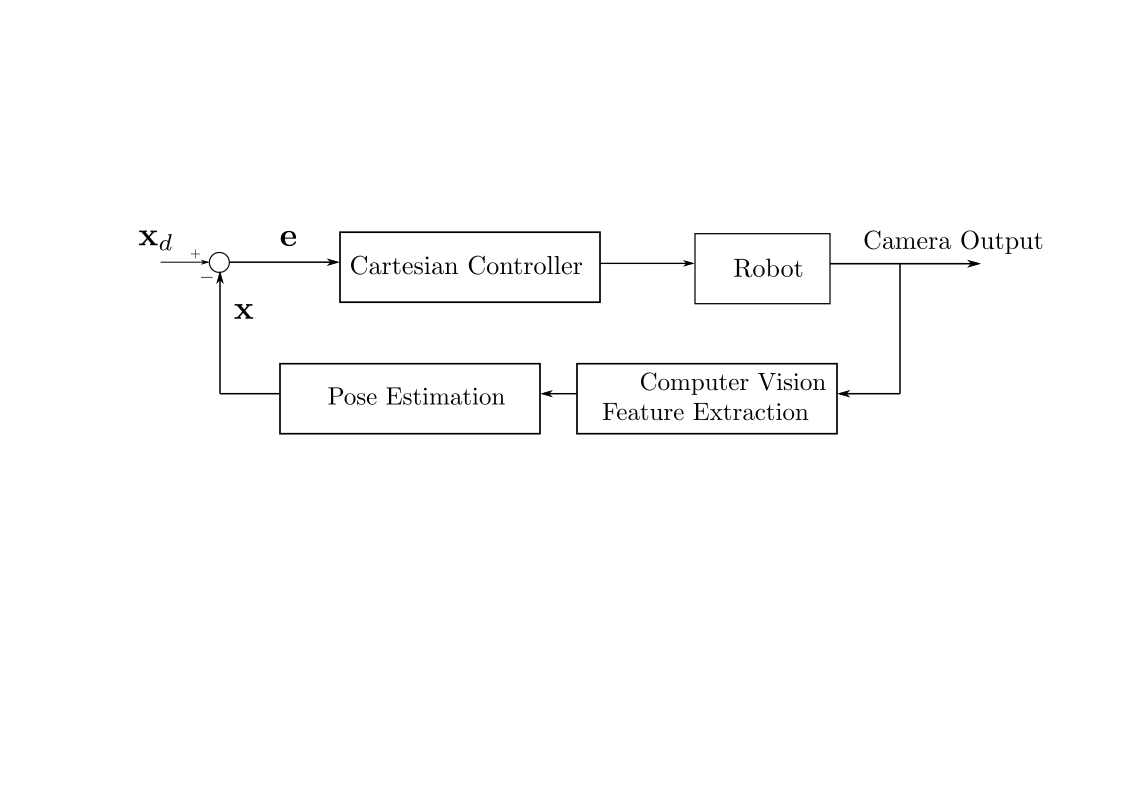
\includegraphics[width=0.6\textwidth]{images/visual-servoing-position-based.png}\\
\caption{Position based visual servoing closed loop control}
\end{figure}
\end{center}

\begin{itemize}
\item \textbf{Photogrammetric technique}
\item \textbf{Stereoscopic vision}: This methodology uses two separate views of the scene from two cameras and calculates the depth of various objects using information from both views. 
\begin{comment}
  For more details about stereoscopic vision see chapter \ref{stereoscopic-vision}
\end{comment}
\item \textbf{Extracting depth from motion} This methodology is very similar to stereoscopic vision and is also known as \textit{monocular} or \textit{motion stereo}. It uses two views from the same camera but from different points in time. A very important assumption for this methodology is to assume that two consecutive views from the video frame do not change significantly, so that some feature points can be matched in both views in order to calculate the depth information. This methodology is cheaper in terms of hardware but it fails to extract depth informations in cases where the robot is completely still.
\item \textbf{Servoing using 3D sensors}
\end{itemize}

\begin{center}
\begin{figure}[htbp]
\centering
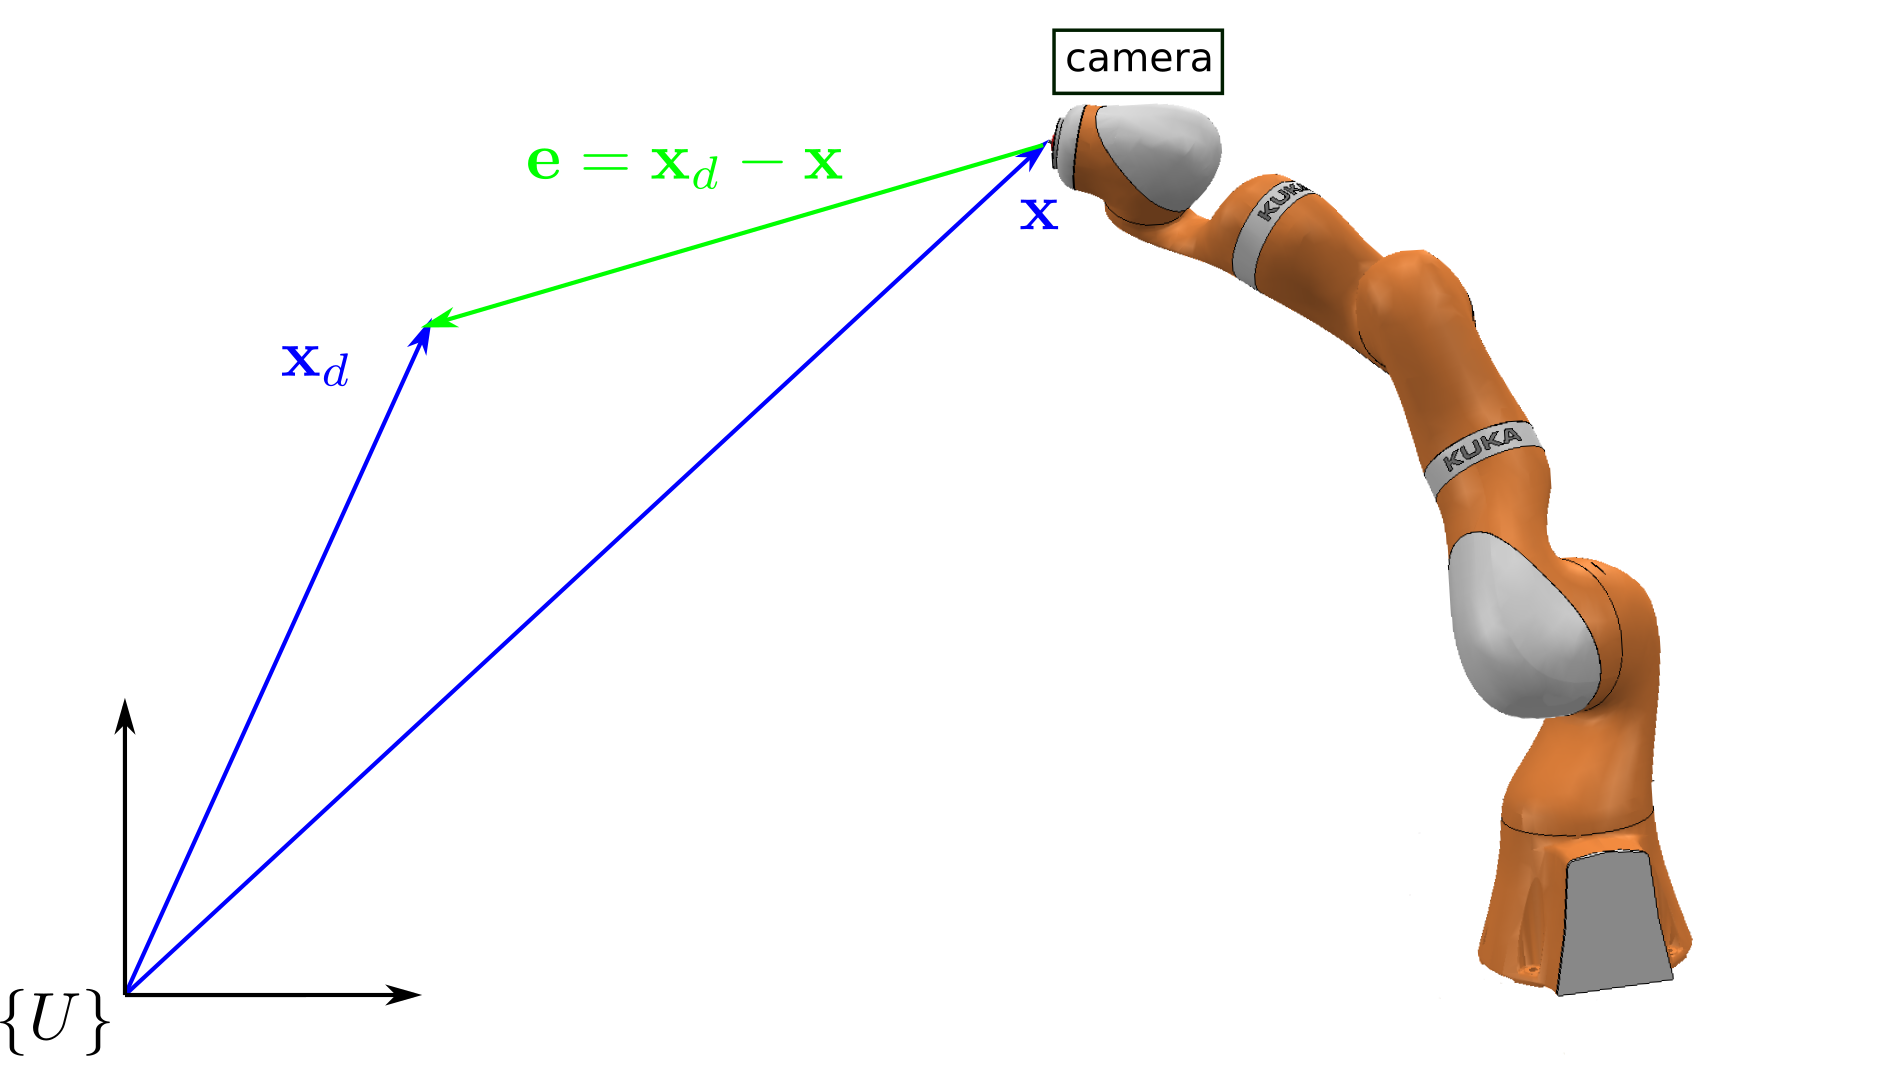
\includegraphics[width=0.6\textwidth]{images/visual-servoing-position-based2.png}\\
\caption{Position based visual servoing using depth from motion, stereo vision or 3D sensors, from which the desired position $\mathbf{x}_d$ is calculated and used to drive the robot.}
\end{figure}
\end{center}

\subsection{Image based servoing}

Image based servoing is a methodology for controlling a robot by directly using features extracted from the image as well as positions on the image plane. The goal of this methodology is to drive the robot in such a way so that the video frame is changed from an initial view to a final, desired view (see Φigure \ref{image-based-servoing-start-end} left and right frames). The commands sent to the robot from this methodology are defined in image space and not in the robot's task space. Moreover the distances calculated in image space are not directly related to distances 
in task space.

\begin{center}
\begin{figure}[htbπ]
\centering
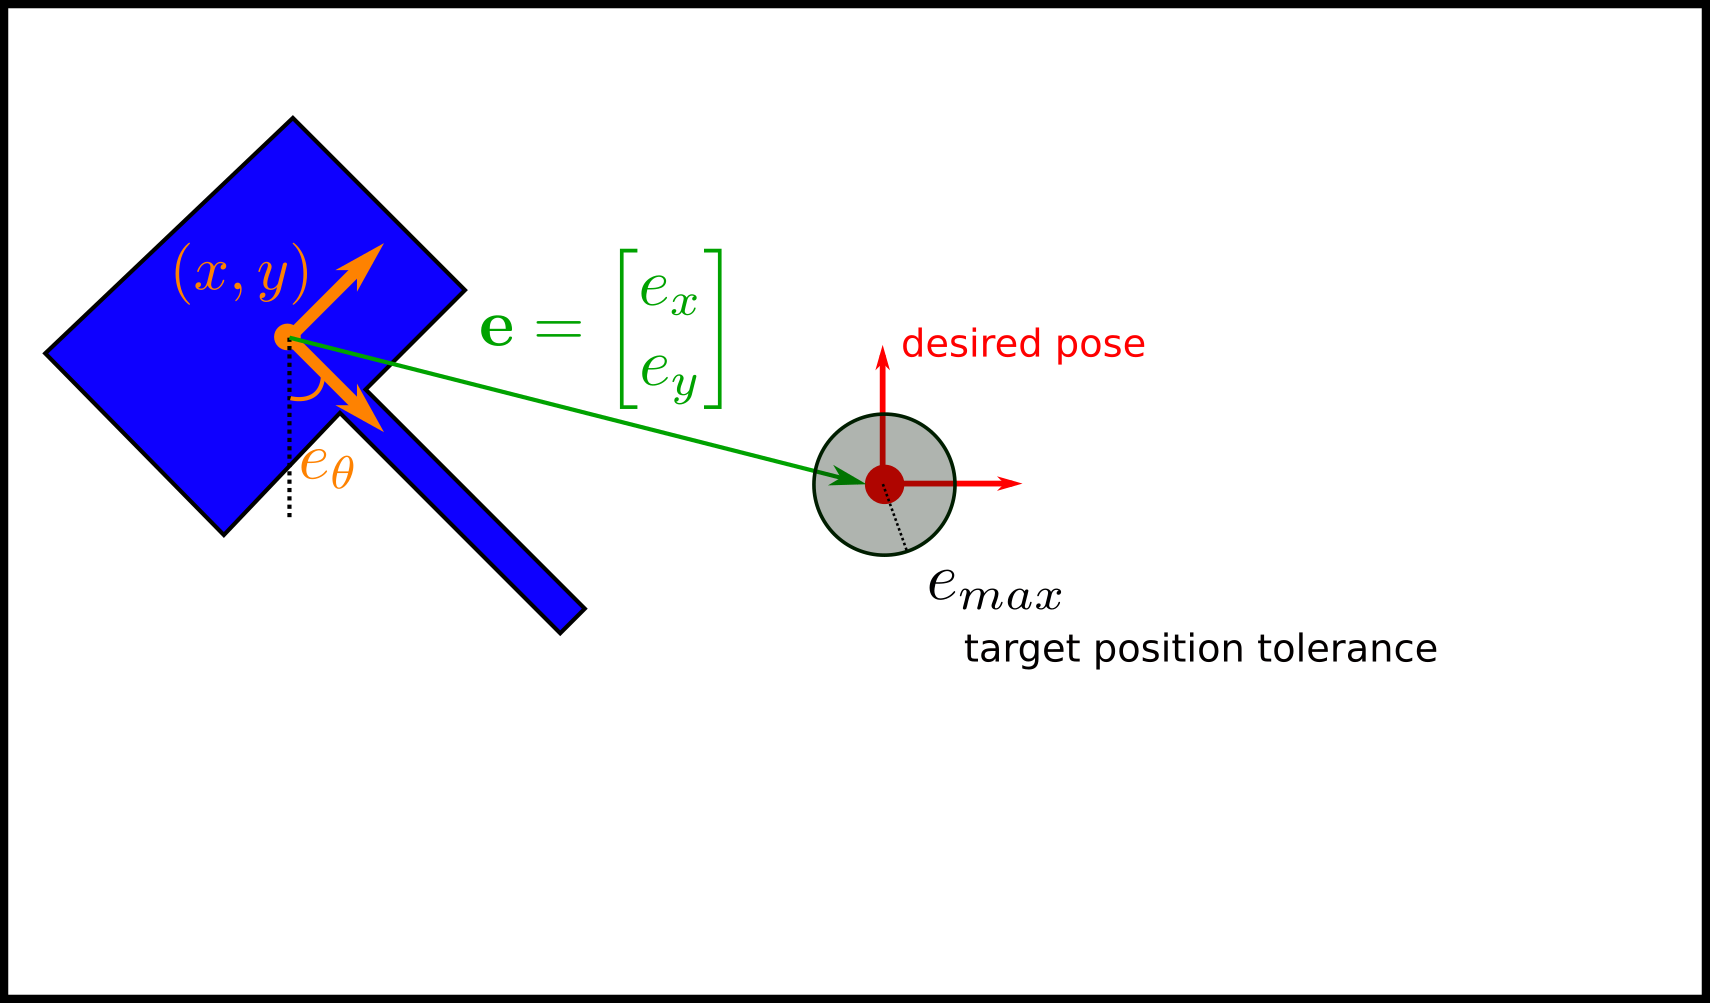
\includegraphics[width=0.35\textwidth]{images/visual_servo_start.png}
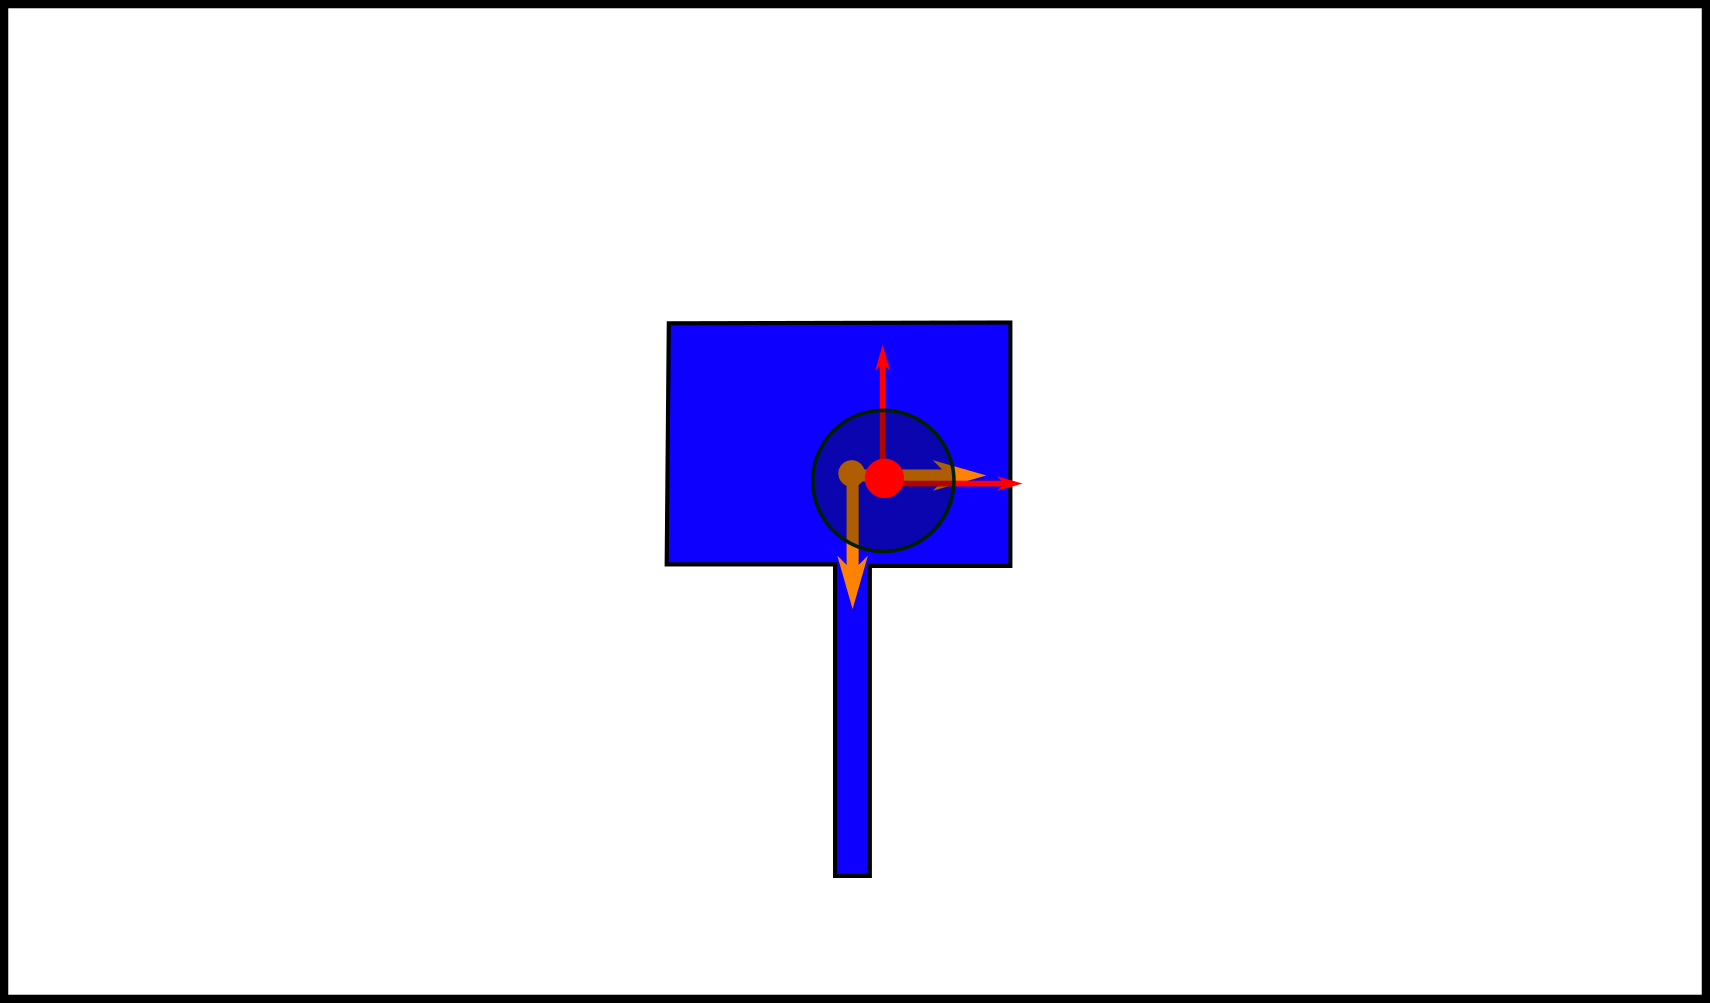
\includegraphics[width=0.35\textwidth]{images/visual_servo_end.png}\\
\caption{Image based visual servoing. The robot arm is controlled using the information gained from the video frames. The frames are 2Dimensional and thus 
the detected objects can have only 3 degrees of freedom which means we can mainly control 3 independent variables, here the $x,y,θ$ variables. The left image 
is the initial frame and the right image is the frame where the object is at the target pose.}
\label{image-based-servoing-start-end}
\end{figure}
\end{center}

The image based visual servoing control system depicted in Figure \ref{visual-servoing-image-based-control} consists of the \textbf{Image Controller}, the \textbf{Plant} (robot) and the \textbf{feedback term}. The Image controller is a simple 
\textbf{PD Controller} which outputs commands to be executed in the plant. These commands are not to be confused with the robot's internal controller commands. These commands are to be used to control the robot in task space, whereas the internal controller drives each joint to the desired angle. The feedback used to calculate the error for the controller, uses the camera's output and based on that it calculates the vector from the detected tool's center of mass to the center of the image frame (feature extraction), as
$
\mathbf{x}[(k+1)T] = \mathbf{x}[kT] + \mathbf{u}[kT], 
$
where $\mathbf{x}[kT] = [x, y, z, θ, φ, ψ]^\top$ and the discrete PID control law is given by equation \ref{discrete-pid-control-law}
\begin{equation}
\label{discrete-pid-control-law}
\mathbf{u}[kT] = K_p \left[ \mathbf{e}[kT] + \frac{T}{T_i} \sum_{i=0}^{k-1} \mathbf{e}[iT] + \frac{T_d}{T} \left( \mathbf{e}[kT] - \mathbf{e}[(k-1)T] \right) \right]
\end{equation}
where $\mathbf{e}[kT] = [e_x, e_y, e_z, e_θ, e_φ, e_ψ]^\top$.

\begin{center}
\begin{figure}[!htb]
\centering

\includegraphics[width=0.8\textwidth]{images/visual-servoing-image-based.png}\\
\caption{Image based visual servoing closed loop control}
\label{visual-servoing-image-based-control}
\end{figure}
\end{center}


\section{Firm grasping algorithm \& Force control}

In order to control the Barrett hand gripper and make sure that the gripper grasps firmly the surgical tool, a hybrid force control scheme must be implemented. This control scheme is hybrid because it combines positions measurements with force measurements. In the context of the Barrett hand, the position of a finger is known using the forward kinematics of the finger's joint angles and the forces are measured using the tactile sensors array which are distributed in the surface of the gripper and the fingers. The proposed force control system is illustrated in the block diagram~\ref{finger-force-control}.

\begin{center}
\begin{figure}[htbp]
\centering
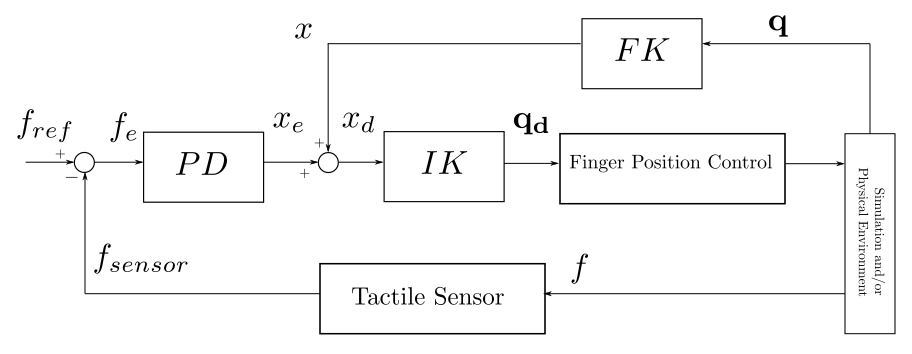
\includegraphics[width=12cm]{images/finger-force-control.png}\\
\caption{Force control on a Barrett Hand gripper finger}
\label{finger-force-control}
\end{figure}
\end{center}

To ensure a firm grasp of the surgical tool, so that it can later be precisely manipulated to do pivot surgical motions, a reference force is required to be defined. The following analysis is for one of the 3 fingers of the gripper and it is the same for all of them. Following the block diagram~\ref{finger-force-control}, if the actual measured force is 0, then the finger is not in contact, which means that there is an error in force. This force error produces a position error via a first PD controller. This position error will be positive and will be added to the current measured position and thus will make the finger move closer to the object. When the finger contacts for the first time the object, then the measured force is non-zero, but it is still less than the desired force that is required for a firm grasp. This means that there is still a force error, which again produces a positions error and again makes the finger move even closer ("squeeze") the object. This control loop repeats until a satisfactory contact is reached and until the desired force is exerted on the object. If the measured force is bigger than the desired value, then the force error is negative and thus a negative position error is generated which in its turn makes the finger to move slightly away from the object, in order to reduce the exerted force. More about force control principles can be found at \url{http://www.osrobotics.org/osr/control/principles.html} as well as an example of force control in ROS and Gazebo at \url{http://www.osrobotics.org/osr/control/examples.html}.